\documentclass{beamer}
\setbeamertemplate{itemize item}[square]
\usepackage{listings,chngcntr}
\usepackage{hyperref}% http://ctan.org/pkg/hyperref
\usepackage{paralist}
%\usepackage{enumitem}% http://ctan.org/pkg/enumitem
\usepackage{amssymb}
\usepackage{amsmath,amsfonts,bm}
\usepackage{amsthm}
\usepackage{url}
\usepackage{algorithm}
\usepackage[noend]{algpseudocode}
\usepackage{indentfirst}
\usepackage[percent]{overpic}
\makeatletter
\def\BState{\State\hskip-\ALG@thistlm}
\makeatother
\usepackage{mathtools}
\usepackage{fancyhdr}
\pagestyle{fancy}
\theoremstyle{definition}
\usepackage{float}
\usepackage{cleveref}
\crefname{section}{§}{§§}
\Crefname{section}{§}{§§}
\newcommand{\R}{\mathbb{R}}
\usepackage{stmaryrd}
\usepackage{graphicx}
\usepackage{caption}
\usepackage{subcaption}
\usepackage[english]{babel}
\usepackage{color}
\newcommand{\hilight}[1]{\colorbox{yellow}{#1}}
\usepackage{soul}
\usepackage{tikz}
\usetikzlibrary{hobby,shapes,arrows,fit,calc,positioning} 
% Choose how your presentation looks.
%
% For more themes, color themes and font themes, see:
% http://deic.uab.es/~iblanes/beamer_gallery/index_by_theme.html
%
\mode<presentation>
{
  \usetheme{Madrid}      % or try Darmstadt, Madrid, Warsaw, ...
  \usecolortheme{default} % or try albatross, beaver, crane, ...
  \usefonttheme{default}  % or try serif, structurebold, ...
  \setbeamertemplate{navigation symbols}{}
  \setbeamertemplate{caption}[numbered]
  \setbeamertemplate{itemize item}[square]
} 


\AtBeginSection[]
{
  \begin{frame}
    \frametitle{Outline}
    \tableofcontents[currentsection, hideallsubsections]
  \end{frame}
}
\usepackage{graphicx}
\usepackage{caption}
\usepackage{subcaption}
\usepackage[english]{babel}
\usepackage[utf8x]{inputenc}
\title[Hierarchical Model Adaptivity]{Hierarchical Model Adaptivity}
\author[GS]{Georgios Sialounas \\{\small Supervised by: Dr T. Pryer,   Dr O. Sutton}}
\institute{MPE CDT}
\date{20 September 2018}

\begin{document}
\pagenumbering{gobble}
\begin{frame}
  \titlepage
\end{frame}




\begin{frame}{Hierarchical Model adaptivity}
\centering
\begin{block}{Definition}
\begin{itemize}
\item Hierarchy of models
\item Adaptivity of models
\end{itemize}
\end{block}
\begin{block}{Hierarchical Stucture}
	\begin{itemize}
	\item  Physical phenomena can be described by various systems of PDEs. 
	\item These models differ in complexity (perhaps \textbf{incrementally})
	\end{itemize}
\end{block}
\end{frame}

\begin{frame}{Hierarchy of models}
\centering
\begin{block}{What is a hierarchy of models?}
Get a complicated model and simplify it using physical reasoning, if possible.  This results in a model hierarchy.
\end{block}
\begin{block}{Example of hierarchical model structure}
	\vspace{-4mm}
 \begin{eqnarray*}
		\textbf{Navier-Stokes Equations:}\quad\quad\,\,\,\textcolor{red}{\frac{D\textbf{u}}{Dt}}\textcolor{blue}{-\Delta \textbf{u}}+\nabla p&=&\textbf{f}\\
		\textbf{Stokes Flow:}\quad\quad\quad\quad \textcolor{blue}{-\Delta \textbf{u}}+\nabla p &=&\textbf{f}\\
	\textbf{Euler Equations: }\quad\quad\quad\quad\textcolor{red}{\frac{D\textbf{u}}{Dt}}+\nabla p&=&\textbf{f}
\end{eqnarray*}
\end{block}
\end{frame}

\begin{frame}{Adaptivity of models}
\centering
\begin{block}{What do we mean by adaptivity of models?}
The capability to choose the PDE system that is most appropriate \textbf{locally}, based on certain criteria as the computation goes on.
\end{block}
\begin{figure}[H]
	\begin{center}
		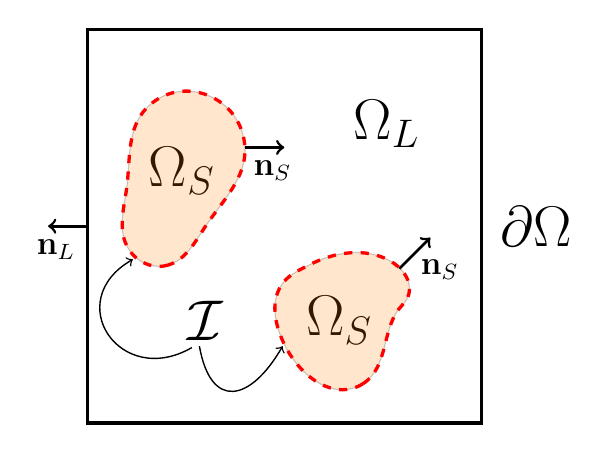
\begin{tikzpicture}
		
		
		\draw[arrows=->,line width=1pt](2,3.5)--(2.5,3.5);
		\draw[arrows=->,line width=1pt](0,2.5)--(-0.5,2.5);
		\node[draw=none,fill=none, xshift = -0.4cm, yshift= 2.2cm] {\large$\textbf{n}_L$}; 
		\node[draw=none,fill=none, xshift = 2.35cm, yshift= 3.2cm] {\large$\textbf{n}_S$}; 
		\node[draw=none,fill=none, xshift = 1.2cm, yshift= 3.2cm] {\huge$\Omega_S$}; 
		\node[draw=none,fill=none, xshift = 3.2cm, yshift= 1.3cm] {\huge$\Omega_S$}; 
		\node[draw=none,fill=none, xshift = 3.8cm, yshift= 3.8cm] {\huge$\Omega_L$}; 
		\node[draw=none,fill=none, xshift = 1.5cm, yshift= 1.3cm] {\huge$\mathcal{I}$}; 
		\node[draw=none,fill=none, xshift = 5.7cm, yshift= 2.5cm] {\huge$\partial\Omega$}; 
		\draw[black, very thick] (0,0)rectangle (5,5);
		
		\node (a) at(1.45, 1.03)  {};
		\node (b) at  (0.7, 2.15){};
		\draw[->,line width =0.5pt] (a)  to [out=-150,in=-150, looseness=2] (b);
		
		\node (c) at(1.4, 1.1)  {};
		\node (d) at  (2.55, 1.1){};
		\draw[->,line width =0.5pt] (c)  to [out=-80,in=600, looseness=2] (d);
		
		\begin{scope}[xshift = 1cm, yshift = 2cm,black]
		\path[draw,use Hobby shortcut,closed=true, fill = orange, opacity = 0.2]
		(0,0) .. (.5,.5) .. (1,1.5) .. (-.25,2) .. (-.5,1) .. (-.5,.25);
		\end{scope}
		\begin{scope}[xshift = 1cm, yshift = 2cm,red, very thick]
		\path[draw,,use Hobby shortcut,closed=true,dashed]
		(0,0) .. (.5,.5) .. (1,1.5) .. (-.25,2) .. (-.5,1) .. (-.5,.25);
		\end{scope}
		
		\draw[arrows=->,line width=1pt](3.96,1.96)--(4.354,2.354);
		\node[draw=none,fill=none, xshift = 4.475cm, yshift= 1.95cm] {\large$\textbf{n}_S$}; 
		\begin{scope}[xshift = 3.5cm, yshift = .5cm,black]	
		\path[draw,use Hobby shortcut,closed=true,fill = orange, opacity = 0.2]
		(0,0) .. (.5,1) .. (.5,1) .. (-0.7,1.5) .. (-1,1.3) .. (-1,.5);
		\end{scope}
		\begin{scope}[xshift = 3.5cm, yshift = .5cm,red, very thick]	
		\path[draw,use Hobby shortcut,closed=true,dashed]
		(0,0) .. (.5,1) .. (.5,1) .. (-0.7,1.5) .. (-1,1.3) .. (-1,.5);
		\end{scope}
		\end{tikzpicture}
	\end{center}
	\caption{A combined problem with different PDE systems in $\Omega_{L}$  and in $\Omega_{S}$.  }
	\label{fig_domain_adapt}
\end{figure}
\end{frame}

\begin{frame}{Hierarchical Model Adaptivity}
\centering
\begin{block}{Definition of \textit{Hierarchical} Model Adaptivity}
A hierarchy of PDE systems modelling a physical phenomenon is created by succesively simplifying the complicated system.	Models are adaptively selected from a hierarchy of models.  
\end{block}
\begin{block}{Further considerations}
		\begin{itemize}
			\item Complicated models are more descriptive but also slower.
			\item Simpler models are faster but contain less detail.
		\end{itemize}
\end{block}

\begin{block}{Research questions}
		\begin{itemize}
			\item How do we couple models?
			\item How do we switch between models (in real-time)?
		\end{itemize}
\end{block}
\end{frame}

\begin{frame}{Combined Stokes-Laplace problem}

\Huge{Combined Stokes-Laplace problem}


\end{frame}


\begin{frame}
\frametitle{Model Problem: Individual Equations }
\begin{block}{Stokes Equations}
	Find $\left(\textbf{u},p\right)$ in $\Omega \subset \mathbb{R}^2$ such that: \vspace{-3mm}\begin{equation}\label{stokes_eq}
	\begin{aligned}
	-\Delta\textbf{u} + \nabla p &= \textbf{f}, \quad \text{in } \Omega \\ 
	\nabla\cdot \textbf{u}&= 0, \quad \text{in } \Omega\\ 
	\textbf{u}|_{\partial\Omega}&=0.
	\end{aligned}
	\end{equation}
\end{block}
\begin{block}{Poisson Equation}
	Find $\textbf{u}$ in $\Omega \subset \mathbb{R}^2$ such that:\vspace{-3mm}
	\begin{equation}\label{laplace_eq}
	\begin{aligned}
	-\Delta\textbf{u} &= \textbf{f}, \quad \text{in } \Omega \\ 
	\textbf{u}|_{\partial\Omega}&=0.
	\end{aligned}
	\end{equation}
\end{block}
The variables $\textbf{u},\, \textbf{f}$ and $p$ represent the velocity, the forcing and the pressure respectively.      
\end{frame}


\begin{frame}{Combined Stokes-Laplace problem}
\begin{block}{ A coupling of the Stokes and Laplace problems}
The Laplace problem is a good approximation to the Stokes problem if the divergence of the velocity is zero or  small.
\end{block}
\begin{figure}[H]
	\begin{center}
		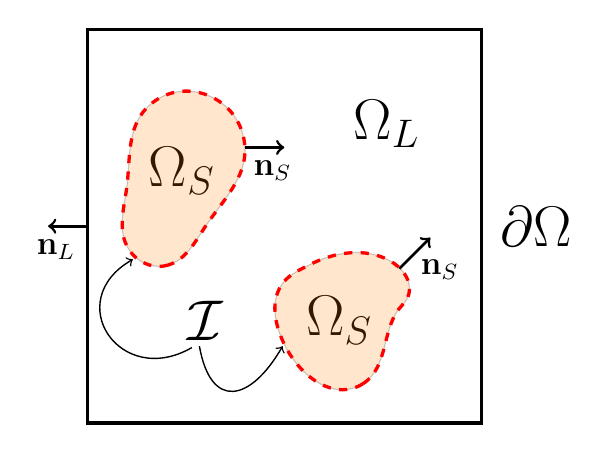
\begin{tikzpicture}
		
		
		\draw[arrows=->,line width=1pt](2,3.5)--(2.5,3.5);
		\draw[arrows=->,line width=1pt](0,2.5)--(-0.5,2.5);
		\node[draw=none,fill=none, xshift = -0.4cm, yshift= 2.2cm] {\large$\textbf{n}_L$}; 
		\node[draw=none,fill=none, xshift = 2.35cm, yshift= 3.2cm] {\large$\textbf{n}_S$}; 
		\node[draw=none,fill=none, xshift = 1.2cm, yshift= 3.2cm] {\huge$\Omega_S$}; 
		\node[draw=none,fill=none, xshift = 3.2cm, yshift= 1.3cm] {\huge$\Omega_S$}; 
		\node[draw=none,fill=none, xshift = 3.8cm, yshift= 3.8cm] {\huge$\Omega_L$}; 
		\node[draw=none,fill=none, xshift = 1.5cm, yshift= 1.3cm] {\huge$\mathcal{I}$}; 
		\node[draw=none,fill=none, xshift = 5.7cm, yshift= 2.5cm] {\huge$\partial\Omega$}; 
		\draw[black, very thick] (0,0)rectangle (5,5);
		
		\node (a) at(1.45, 1.03)  {};
		\node (b) at  (0.7, 2.15){};
		\draw[->,line width =0.5pt] (a)  to [out=-150,in=-150, looseness=2] (b);
		
		\node (c) at(1.4, 1.1)  {};
		\node (d) at  (2.55, 1.1){};
		\draw[->,line width =0.5pt] (c)  to [out=-80,in=600, looseness=2] (d);
		
		\begin{scope}[xshift = 1cm, yshift = 2cm,black]
		\path[draw,use Hobby shortcut,closed=true, fill = orange, opacity = 0.2]
		(0,0) .. (.5,.5) .. (1,1.5) .. (-.25,2) .. (-.5,1) .. (-.5,.25);
		\end{scope}
		\begin{scope}[xshift = 1cm, yshift = 2cm,red, very thick]
		\path[draw,,use Hobby shortcut,closed=true,dashed]
		(0,0) .. (.5,.5) .. (1,1.5) .. (-.25,2) .. (-.5,1) .. (-.5,.25);
		\end{scope}
		
		\draw[arrows=->,line width=1pt](3.96,1.96)--(4.354,2.354);
		\node[draw=none,fill=none, xshift = 4.475cm, yshift= 1.95cm] {\large$\textbf{n}_S$}; 
		\begin{scope}[xshift = 3.5cm, yshift = .5cm,black]	
		\path[draw,use Hobby shortcut,closed=true,fill = orange, opacity = 0.2]
		(0,0) .. (.5,1) .. (.5,1) .. (-0.7,1.5) .. (-1,1.3) .. (-1,.5);
		\end{scope}
		\begin{scope}[xshift = 3.5cm, yshift = .5cm,red, very thick]	
		\path[draw,use Hobby shortcut,closed=true,dashed]
		(0,0) .. (.5,1) .. (.5,1) .. (-0.7,1.5) .. (-1,1.3) .. (-1,.5);
		\end{scope}
		\end{tikzpicture}
	\end{center}
	\caption{The combined Stokes-Laplace problem with the Stokes equation in $\Omega_S$ and Laplace's Equation in $\Omega_L$}
	\label{combi}
\end{figure}
\end{frame}


  \begin{frame}{Finite Element Method}
  \begin{block}{What does the FEM do?}
  \begin{itemize}
\item Approximates the PDE
\item Approximates the solution's Function Space
\item Translate our problem into a finite-dimensional linear algebra problem
\item Can approximate very complicated domains
  \end{itemize}
  \end{block}

\begin{block}{Weak Formulation}
Multiply our problem by a test function and integrate by parts.  This is the weak form of the problem.
\end{block}
\end{frame}


\begin{frame}
\frametitle{Model Problem: Individual Weak Formulations}
\begin{block}{Stokes Equations Weak form}\vspace{-0mm}
	\begin{equation*}\label{weak_stokes_1_ind}
	\begin{rcases}
	\small{\begin{aligned}
		\int_{\Omega}\nabla \textbf{u} : \nabla \textbf{v}-p\left(\nabla \cdot \textbf{v}\right)  &=\int_{\Omega}\textbf{f}\cdot \textbf{v}  \quad \forall  \textbf{v}\in \mathbb{V}\\
		\int_{\Omega}q\left(\nabla \cdot \textbf{u}\right) &= 0\quad\quad\quad\,\,\, \forall q\in \mathbb{P},
		\end{aligned}}
	\end{rcases}\text{ in }\Omega
	\end{equation*}
\end{block}
\begin{block}{Laplace's Equation Weak form}
	\begin{equation*}\label{weak_poisson_ind}
	\int_{\Omega}\nabla \textbf{u} : \nabla \textbf{v} = 
	\int_{\Omega}\textbf{f}\cdot \textbf{v}  \quad \forall  \textbf{v}\in \mathbb{V}\quad\text{ in } \Omega.
	\end{equation*}
\end{block}
\end{frame}


  \begin{frame}
  \frametitle{Model Problem: Combined Weak Formulation}
  \begin{block}{Stokes Equation Weak form in $\Omega_S$}\vspace{-4mm}
  \begin{equation*}\label{weak_stokes_1}
  \small{\begin{aligned}
  	\int_{\Omega_S}\nabla \textbf{u}_S : \nabla \textbf{v}_S-p\left(\nabla \cdot \textbf{v}_S\right) +\int_{\mathcal{I}} \left(pI \textbf{n}_S-\nabla\textbf{u}_S\textbf{n}_S\right)\cdot \textbf{v}_S &=\int_{\Omega_S}\textbf{f}\cdot \textbf{v}_S  \quad \forall  \textbf{v}\in \mathbb{V}_S\\
  	\int_{\Omega_S}q\left(\nabla \cdot \textbf{u}_S\right) &= 0\quad\quad\quad\,\,\quad \forall q\in \mathbb{P}.
  	\end{aligned}}
  \end{equation*}
  \end{block}
\begin{block}{Laplace's Equation Weak form in $\Omega_L$}
\begin{equation*}\label{weak_poisson}
\int_{\Omega_L}\nabla \textbf{u}_L : \nabla \textbf{v}_L - \int_{\mathcal{I}} \textbf{v}_L \cdot \left(\nabla\textbf{u}_L\textbf{n}_L\right)= 
\int_{\Omega_L}\textbf{f}\cdot \textbf{v}_L  \quad \forall  \textbf{v}_L\in \mathbb{V}_L.
\end{equation*}
\end{block}

  \end{frame}



\begin{frame}
\frametitle{Combined Weak form}
	\begin{block}{Weak form for combined problem}\vspace{-4mm}
	\begin{equation}\label{weak_total}{\small
	\begin{aligned}
	\int_{\Omega}\nabla \textbf{u} : \nabla \textbf{v}-\int_{\Omega_S}p\left(\nabla \cdot \textbf{v}\right) +\int_{\mathcal{I}}\left( pI \textbf{n}_S-\llbracket\nabla\textbf{u}\rrbracket\right)\cdot\textbf{v} &=\int_{\Omega}\textbf{f}\cdot \textbf{v} \quad \forall  \textbf{v}\in \mathbb{V}\\
	\int_{\Omega_S}q\left(\nabla \cdot \textbf{u}\right) &= 0\quad\quad\,\,\,\quad \forall q\in \mathbb{P},
	\end{aligned}}
	\end{equation}
	\end{block}
where the jump accross $\mathcal{I}$ is given by:\vspace{-2mm}
\begin{equation}
\llbracket\nabla \textbf{u} \rrbracket \coloneqq \textbf{n}_S\cdot\nabla \textbf{u}_S+\textbf{n}_L\cdot  \nabla\textbf{u}_L.
\end{equation}
\end{frame}
 
\begin{frame}
\frametitle{Does my problem have a solution?}
\vspace{0mm}
\begin{block}{\textit{inf-sup} conditions}
A problem is well-posed if  it accepts a unique solution which is also stable - e.g. that can be controlled by the problem data (see \cite{hadamard1932probleme}). Inf-sup conditions are necesary and sufficient conditions for our problem to be well-posed (see \cite{ern2013theory}).   This condition, for an abstract variational problem is
\begin{eqnarray}\label{coerc_a}
\inf_{\textbf{u}\in \mathbb{V}}\sup_{\textbf{v}\in \mathbb{V}}\frac{a\left(\textbf{u},\textbf{v}\right)}{\left|\textbf{u}\right|_1 \left|\textbf{v}\right|_1}&\geq&\alpha>0
\end{eqnarray}
\end{block}

\begin{block}{Solvability Condition}
For the \textit{inf-sup} conditions to hold in this case, we require that on $\mathcal{I}$\vspace{-5mm}
\begin{equation}
\int_{\mathcal{I}}\left(pI \textbf{n}_S- \llbracket \nabla \textbf{u}\rrbracket\right)\cdot\textbf{v}=0.
\end{equation}
\end{block}
\end{frame}
    \begin{frame}{Implementation of Adaptivity}

\begin{block}{Model and Mesh Adaptivity}
Model and Mesh Adaptivity are driven by an a-posteriori error indicator.  This is a quantity that can be computed from available information
\end{block}

\begin{block}{The a-posteriori error indicator}
\begin{equation*}\small\label{approach1_indicator}
\small{\eta_{R,K}=\begin{cases}
	\left(h^2_K\left|\left|\textbf{f}_T+\Delta \textbf{u}_T-\nabla p_T\right|\right|^2_K+\left|\left|\text{div} \textbf{u}_T\right|\right|^2_K+\frac{1}{2}\sum_{E\in\mathcal{E}_{K,\Omega}\setminus\mathcal{I}}h_E\left|\left| \llbracket \nabla \textbf{u}_T -p_T \rrbracket \right|\right|_E^2\right)^{1/2} \text{ if }K\in\Omega_S,\\
	\left(h^2_K\left|\left|\textbf{f}_T+\Delta \textbf{u}_T\right|\right|^2_K+\frac{1}{2}\sum_{E\in\mathcal{E}_{K,\Omega}\setminus\mathcal{I}}h_E\left|\left| \llbracket \nabla \textbf{u}_T  \rrbracket \right|\right|_E^2\right)^{1/2}\text{ if }K\in\Omega_L
	\end{cases}}
\end{equation*}
\end{block}
We implement model and mesh adaptivity by breaking the indicator into a \textbf{modelling error}  and a \textbf{discretisation error}.
    \end{frame}
  \begin{frame}{Numerical Simulations}
  \centering
  \huge{Numerical simulations}
  \end{frame}
 \begin{frame}
 \frametitle{Simulations: Analytical Solution}
 \begin{block}{How do we check that our model works?}
We manufacture a solution and use it on a simple problem.
 \end{block}
 \begin{block}{Analytical Solution}
 	
 	 \begin{eqnarray}
 	\label{benchmark_u}
 	\textbf{u}\left(\textbf{x}\right)&=&\begin{bmatrix}
 	200x^2\left(1-x\right)^2y\left(1-y\right)\left(1-2y\right)  \\
 	-200y^2\left(1-y\right)^2x\left(1-x\right)\left(1-2x\right)  
 	\end{bmatrix} \text{ and}\\\label{benchmark_p}
 	p &=& x\left(x-0.5\right)\left(x-1\right)\left(y^3-1.5y^2+0.625y-0.0625\right)
 	\end{eqnarray}
 \end{block}
\end{frame}

\begin{frame}
\frametitle{Simulations:  Stokes Solution}
\vspace{-8mm}
\begin{figure}[H]
	\centering
	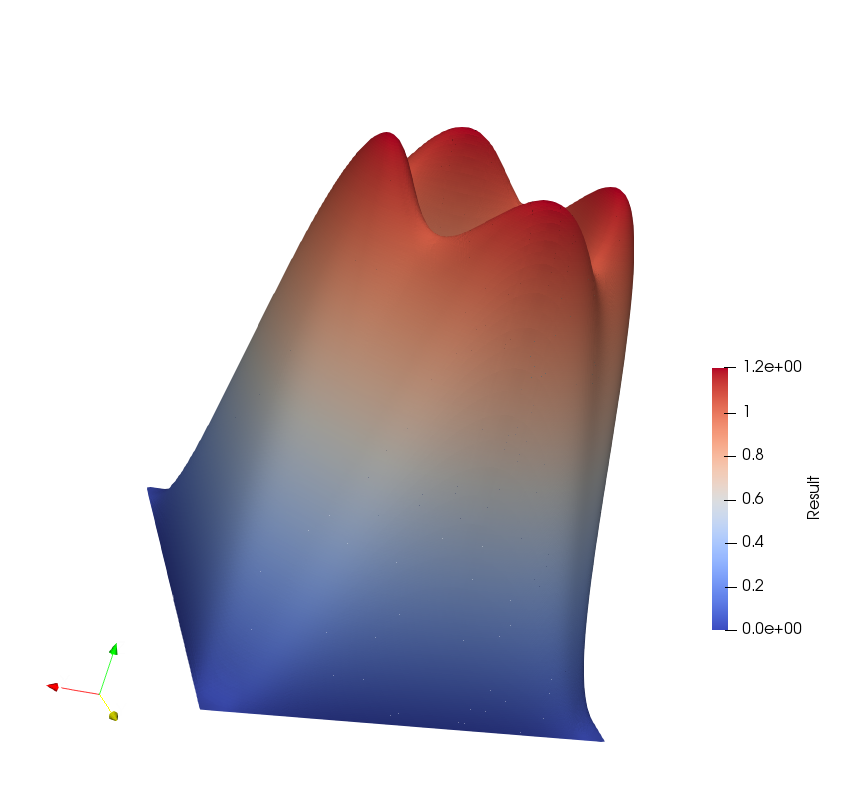
\includegraphics[width=7cm]{stokes_cg_velocities}
	\caption{Stokes velocity magnitude}
	\label{fig_stokes_sol}
\end{figure}
\end{frame}  
\begin{frame}
\frametitle{Simulations: Stokes with Laplace}

\begin{figure}
	\centering
	\begin{minipage}{0.5\textwidth}
		\centering
		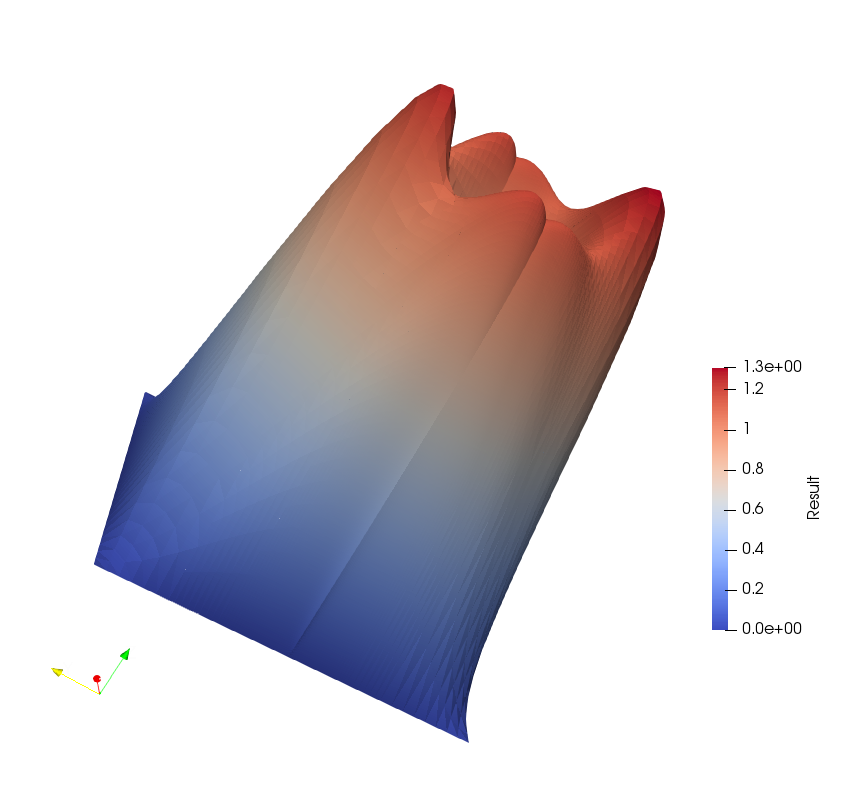
\includegraphics[width=1\linewidth]{combi_u}
		\captionof{figure}{Velocity Mangitude}
		\label{fig:test1}
	\end{minipage}%
	\begin{minipage}{.55\textwidth}
		\hspace{-10mm}
		\vspace{5mm}
		\centering
		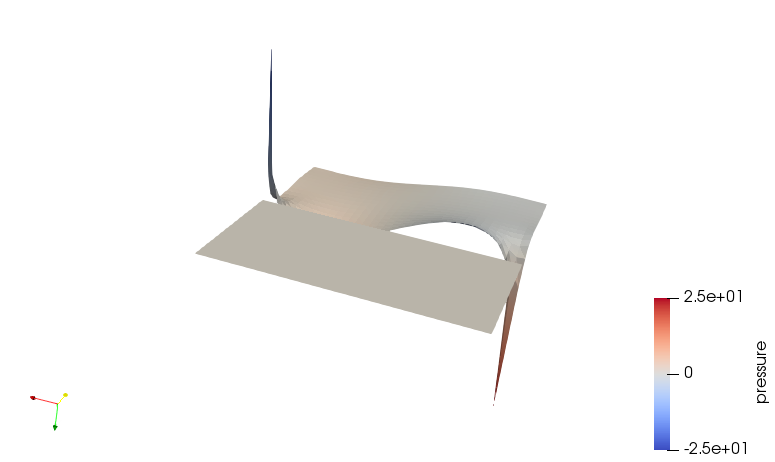
\includegraphics[width=1\linewidth]{combi_p}
		\captionof{figure}{Pressure}
		\label{fig:test2}
	\end{minipage}
\end{figure}
\end{frame}    

%\begin{frame}{Convergence for combined Stokes-Laplace}
%\begin{table}[H]
%	\begin{center}
%	\resizebox{\textwidth}{!}{	\begin{tabular}{|c|c|c|c|c|c|} \hline
%			refinement cycle & cells & dofs & $||p-p_h||_{L^2}$ & $||u-u_h||_{L^2}$ & $||u-u_h||_{Hdiv}$\\ \h%line
	%		0 & 1024 & 20963 & 1.1118e+00 & 0.0964 & 0.4363\\ \hline
	%		1 & 2128 & 44039 & 1.1123e+00 & 0.0964 & 0.4360\\ \hline
	%		2 & 4408 & 91583 & 1.1125e+00 & 0.0964 & 0.4359\\ \hline
	%		3 & 9268 & 192207 & 1.1126e+00 & 0.0964 & 0.4359\\ \hline
	%		4 & 19480 & 403647 & 1.1126e+00 & 0.0964 & 0.4359\\ \hline
%	\end{tabular}}
		%\caption{Convergence for $\textbf{u}$ and $p$ in different norms for the combined model with a fixed interface.}
		%\label{tablebenchmark_convergence_mm1}
	%\end{center}
%\end{table}
%\end{frame}

\begin{frame}
\frametitle{Future-steps/Questions?}
\begin{block}{Future steps}
	\begin{itemize}
\item Identify the reason for the non-zero velocity gradient jump
\item Model Mesh adaptivity with non-fixed domains
\item Try a different model hierarchy
	\end{itemize}
\end{block}
\centering
Thank you! Questions?
\end{frame}


\begin{frame}[allowframebreaks]
\frametitle{References}
\bibliography{biblio_draft}
\bibliographystyle{ieeetr}
\end{frame}
\end{document}
